\section{Lexikalische Elemente}	
	\subsection{Bezeichner/Namen}
		\begin{minipage}[t]{5.5 cm}
			Bezeichner bezeichnen in einem \lc{C++} Programm:
			 	\begin{compactitem}
					\item Variablen
					\item Funktionen
					\item selbst definierte Datentypen
					\item Klassen
					\item Objekte
					\item ...
			 	\end{compactitem}
		\end{minipage}
		\hspace*{0.5cm}
		\begin{minipage}[t]{5 cm}
			 Bezeichner k�nnen bestehen aus:
				\begin{compactitem}
					\item Buchstaben a-z, A-Z
					\item Ziffern 0-9
					\item Underscore \_
				\end{compactitem}
			Das erste Zeichen eines Bezeichners darf keine Ziffer sein!
		\end{minipage}
		\hspace*{1.0cm}
		\begin{minipage}[t]{6 cm}
			Styleguide Variablen \& Funktionen:
				\begin{compactitem}
					\item mit Kleinbuchstaben beginnen	 			
					\item erster Buchstaben von zusammengesetzten W�rtern ist gross	
					\item keine Underscores
				\end{compactitem}
				\vspace*{0.2cm} 
				Beispiele: \lc{counter}, \lc{maxSpeed}, \lc{getCount()}, \lc{setMaxSpeed()}, \\ \lc{init()},	
		\end{minipage}	
	
	\subsection{Schl�sselw�rter}
	Schl�sselw�rter sind reservierte Bezeichner mit einer vorgegebenen Bedeutung und dienen zur Beschreibung von Aktionen und Objekten in \lc{C++} Programmen. Sie d�rfen daher nicht anderweitig verwendet werden.\\
	
		\vspace*{-0.4cm}
		\begin{minipage}[t]{3.6 cm}
			\begin{compactitem}
		 		\item \lc{asm}
		 		\item \lc{auto}				
		 		\item \lc{bool}
		 		\item \lc{break}
		 		\item \lc{case}
		 		\item \lc{catch}
		 		\item \lc{char}
		 		\item \lc{class}
		 		\item \lc{const}
				\item \lc{const\_cast}
		 		\item \lc{continue}
		 		\item \lc{default}
		 		\item \lc{delete}
		 	\end{compactitem}
	 	\end{minipage}
	 	\begin{minipage}[t]{3.6 cm}
		 	\begin{compactitem}	
		 		\item \lc{do}
		 		\item \lc{double}
		 		\item \lc{dynamic\_cast}
		 		\item \lc{else} 
		 		\item \lc{enum}			
		 		\item \lc{explicit}
		 		\item \lc{extern}	
		 		\item \lc{false}
		 		\item \lc{float}
		 		\item \lc{for}
		 		\item \lc{friend}
		 		\item \lc{goto} 
		 		\item \lc{if}	 			
		 	\end{compactitem}
	 	\end{minipage}
	 	\begin{minipage}[t]{4.4 cm}
		 	\begin{compactitem}					
		 		\item \lc{inline}
		 		\item \lc{int}
		 		\item \lc{long}
		 		\item \lc{mutable}	
		 		\item \lc{namespace}
		 		\item \lc{new}
		 		\item \lc{operator}	 
		 		\item \lc{private}				
		 		\item \lc{protected}
		 		\item \lc{public}
		 		\item \lc{register}
		 		\item \lc{reinterpret\_cast}
		 		\item \lc{return}			
		 	\end{compactitem}
	 	\end{minipage}
	 	\begin{minipage}[t]{3.6 cm}
		 	\begin{compactitem}	
		 		\item \lc{short}	
		 		\item \lc{signed}
		 		\item \lc{sizeof}				
		 		\item \lc{static}
		 		\item \lc{static\_cast}		 	
		 		\item \lc{struct}
		 		\item \lc{switch}
		 		\item \lc{template}
		 		\item \lc{this}
		 		\item \lc{throw}
		 		\item \lc{true}	
		 		\item \lc{try}
		 		\item \lc{typedef}
		 	\end{compactitem}
	 	\end{minipage}
	 	\begin{minipage}[t]{3.6 cm}
		 	\begin{compactitem}	 
		 		\item \lc{typeid}
		 		\item \lc{typename}
		 		\item \lc{union} 
		 		\item \lc{unsigned}
		 		\item \lc{using} 
		 		\item \lc{virtual}				
		 		\item \lc{void}
		 		\item \lc{volatile}	
		 		\item \lc{wchar\_t}
		 		\item \lc{while}				 			
		 	\end{compactitem}
	 	\end{minipage}
 		
		\subsubsection{Zeichenketten}
		\begin{minipage}[t]{9 cm}
			Ein Zeichenketten-Literal ist eine (m�glicherweise auch leere) Sequenz von Zeichen, die in doppelten Hochkommas eingeschlossen ist. \\
			\lc{"Hallo"}, \lc{""} (leere Zeichenkette), \lc{"Ha \textbackslash x41"} (Ha A), ... 
		\end{minipage}
		\hspace*{1cm}
		\begin{minipage}[t]{9 cm}
			Beispiel \lc{"Ritchie"}\\
 			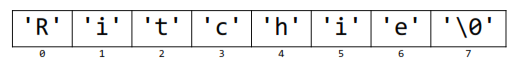
\includegraphics[width=0.6\textwidth]{pics/Zeichenkonstante.png}
 		\end{minipage}		
	\subsection{Operatoren und Begrenzer \verweiscpp{3.5}}
		Operatoren und Begrenzer sind einzelne Sonderzeichen bzw. Sequenzen von Sonderzeichen oder reservierten W�rter mit vordefinierter Bedeutung. Operatoren bestimmen Aktionen, die auf Programmobjekte ausgef�hrt werden k�nnen. Begrenzer wiederum trennen Symbole des Programmtexts voneinander.
	
	\subsection{Kommentare}
		\begin{minipage}[t]{13.5 cm}
			Kommentare sind Anmerkungen im Programmtext, die f�r den Leser bestimmt sind. Der Compiler ignoriert sie und entfernt sie vor dem �bersetzen des Programms in Maschinencode aus dem Quelltext.
		\end{minipage}
		\hspace*{1cm}
		\begin{minipage}[t]{4.5 cm}
			\lc{//} Einzeilige Kommentare \\
			\lc{/* */} Kommentare �ber \newline
			\phantom{} \ \ \ \ \ \ \ \ \ mehrere Zeilen
		\end{minipage}